\documentclass[11pt]{exam}
\usepackage[margin=1in]{geometry}
\pagestyle{plain}
\usepackage{amsmath,amsfonts,amssymb,amsthm,enumerate}
\usepackage{multicol}
\usepackage[]{graphicx}
\usepackage{hyperref}
\usepackage{tikz}
\usepackage{pgfplots}
\usepackage{subfigure}
\usepackage[final]{pdfpages}

\addtolength{\footskip}{2\baselineskip} % to lower the page numbers
\title{\vspace{-0.5in} Math 115 \\ Worksheet Section 3.4}
\date{}


% \theoremstyle{definition}
% \newtheorem{problem}{Problem}
\renewcommand{\questionlabel}{\textbf{Problem~\thequestion.}}
%\printanswers

\begin{document}
\maketitle
\vspace{-0.75in}
\begin{questions}
  \question
    \begin{parts}
    \part Suppose the squirrel population in my neighborhood grows
      based on acorn availability, at a rate of 2 squirrels per
      bushel.  Acorn availability is currently growing at a rate of 5
      bushels per week.  How fast are the squirrels taking over my
      neighborhood?
    \part Now suppose that a better model is $$s(a(t))= 2(a(t))^2
= 2\left(\sin\left(\frac{\pi}{6}t\right)+3\right)^2.$$ How fast are
the squirrels taking over my neighborhood with this model?
    \end{parts}
    \begin{solution}
      \begin{enumerate}[(a)]
      \item \(5\) bushels per week \(\times\) \(2\) squirrels per
        bushel \(=\) \(10\) squirrels per week.
      \item \(\frac{d}{dt}(s(a(t))) = s'(a(t)) \cdot
        a'(t)\). Furthermore, we know \(s(a) = 2a^2\), so \(s'(a) =
        4a\) and \(a(t) = \sin\left( \frac{\pi}{6}t \right)+3\), so
        \(a'(t) = \cos\left( \frac{\pi}{6}t \right)\cdot \left(
          \frac{\pi}{6} \right)\) (via another chain rule
        application). Thus, putting it all together \[
\frac{d}{dt}(s(a(t))) = s'(a(t)) \cdot
        a'(t) = 4(a(t)) \cdot a'(t) = 4\left( \sin\left(
            \frac{\pi}{6}t \right)+3 \right) \cdot \left(\frac{\pi}{6}\cos\left( \frac{\pi}{6}t \right) \right)
        \]
      \end{enumerate}
    \end{solution}
\question Find the derivatives of the following.
  \begin{parts}
  \part $y=\tan\left(\frac{x}{2}\right)$
  \part $y= \sqrt{e^{-3t^2}+5}$
  \part \(f(x)=(2x+1)^{10}(3x-1)^7\)
  \end{parts}
  \begin{solution}
    \begin{enumerate}[(a)]
    \item \(y' = \frac{1}{\cos^2(x/2)}\cdot \left( \frac{1}{2} \right)
      = \frac{1}{2\cos^2(x/2)}\). This can also be written as \(\frac{1}{2}\sec^2\left( \frac{x}{2} \right)\).
    \item \(y' = \frac{1}{2}\left( e^{-3t^2}+5 \right)^{-1/2}\cdot\left(
        e^{-3t^2}(-6t) \right) = -3te^{-3t^2}\left( e^{-3t^2}+5 \right)^{-1/2}\)
    \item \(f'(x) = 10(2x+1)^9 \cdot 2 \cdot (3x-1)^7 + (2x+1)^{10} \cdot
      7(3x-1)^6 \cdot 3\)
    \end{enumerate}
  \end{solution}
\question A yam is put into a 200$^{\circ}$C oven.  Newton's law of cooling (and warming) tells us that its temperature $T$ after $t$ minutes is
$$T(t) = 200 - ae^{-bt}$$
for some constants $a$ and $b$. After $30$ minutes, the temperature of the yam is 120$^{\circ}$C and increasing at an instantaneous rate of 2$^{\circ}$C per minute.  Find $a$ and $b$. 
\begin{solution}
  From the problem, we know \(T(30) = 120\) and
  \(T'(30)=2\). Furthermore, we can compute \[
    T'(t) = -a e^{-bt} \cdot (-b) = ab e^{-bt}
  \]
  Thus, we need to solve, at \(t=30\), \[
    \begin{cases}
      120 = T(30) = 200-ae^{-30b}\\
      2 = T'(30) = abe^{-30b}
    \end{cases}
  \]
  From the first equation, we can deduce
  \begin{align*}
    120 = 200-ae^{-30b} & \implies 80 = ae^{-30b} \\
    & \implies \frac{80}{a} = e^{-30b}
  \end{align*}
  which is valid since we know \(a\) cannot be \(0\). Substituting
  into the second equation, we get \[
    2 = ab \frac{80}{a} = 80b \implies b = \frac{1}{40}
  \]
  Therefore, \(a = 80 e^{30/40} = 80 e^{3/4}\).
\end{solution}
\question Prove the quotient rule by writing \(h(x) =
  f(x)(g(x))^{-1}\) and taking the derivative using the product rule
  and the chain rule. Show your work carefully!
\question (Fall 2016 Exam 2) % problem 1
The table below gives several values for the function $f$ and its derivative $f'$. You may assume that $f$ is invertible and differentiable.
\begin{center}
  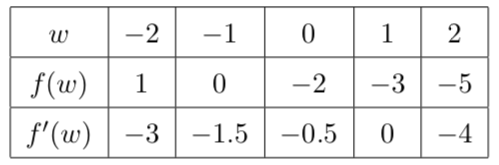
\includegraphics[scale=0.4]{Figures/table2.png}
\end{center}
	For each of the parts below, find the exact value of the given quantity. If there is not enough information provided to find the value, write \emph{not enough info}. If the value does not exist, write \emph{does not exist}. You are not required to show your work on this problem. However, limited partial credit may be awarded based on work shown.
	\begin{multicols}{2}
	\begin{enumerate}[(a)]
	\item Let $h(w) = \frac{f(w)}{6+w}$. Find $h'(-2)$.
	\item Let $k(w) = 3^{f(2w)}$. Find $k'(-1)$.
	\item Let $p(w) = f(f(-w+1))$. Find $p'(1)$.
	\item Let $r(w) = w (f(w))^2$. Find $r'(2)$.
	\end{enumerate}
	\end{multicols}
        \begin{solution}
          See \href{https://dhsp.math.lsa.umich.edu/exams/115exam2/f16/s1.pdf}{https://dhsp.math.lsa.umich.edu/exams/115exam2/f16/s1.pdf}
        \end{solution}
\question Use the chain rule to prove \(\frac{d}{dx}(\ln(x)) =
  \frac{1}{x}\) by writing \(e^{\ln(x)} = x\) and taking the
  derivative of both sides.
\question (Winter 2017 Exam 2) % problem 4
  A portion of the graph of the function $w(x)$ is shown below.
  \begin{center}
    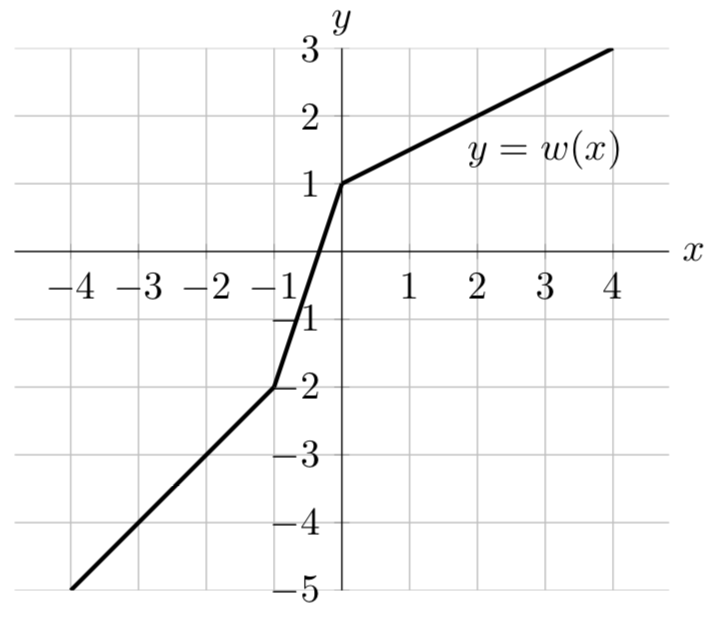
\includegraphics[scale=0.6]{Figures/graphw.png}
  \end{center}
	For each of the parts below, find the value of the given quantity. If there is not enough information provided to find the value, write \emph{not enough info}. If the value does not exist, write \emph{does not exist}. You are not required to show your work on this problem. However, limited partial credit
may be awarded based on work shown. All your
answers must be in exact form.
	\begin{enumerate}[(a)]
		\item Let $h(u) = \ln(3w(u))$. Find the value of $h'(1)$.
		\item Let $n(x) = \frac{w(x)}{1-x^2}$. Find $n'(-2)$.
		\item Let $s(x)$ be the exponential function $s(x) = 4^{w(x)}$. Find $s'(2)$.
	\end{enumerate}
        \begin{solution}
          See \href{https://dhsp.math.lsa.umich.edu/exams/115exam2/w17/s4.pdf}{https://dhsp.math.lsa.umich.edu/exams/115exam2/w17/s4.pdf}
        \end{solution}
\question (Winter 2016 Exam 2) Let $f$ be the piecewise linear function with graph shown below.

\begin{multicols}{2}
  \begin{center}
    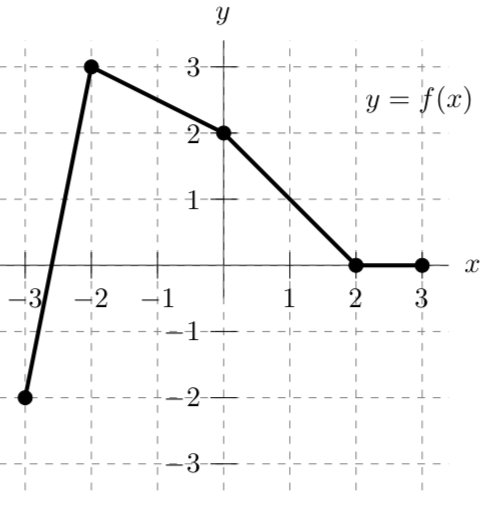
\includegraphics[scale=0.4]{Figures/graph4.png}
  \end{center}
	\noindent
	The table below gives several values of a differentiable function g and its derivative $g'$.
Assume that both $g(x)$ and $g'(x)$ are invertible.
\begin{center}
  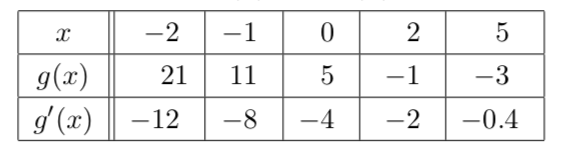
\includegraphics[scale=0.4]{Figures/table4.png}
\end{center}
	\noindent
	For each of parts below, find the value of the given quantity. If there is not enough information provided to find the value, write \emph{not enough info}. If the value does not exist, write \emph{does not exist}.
	\end{multicols}
	\begin{multicols}{2}
	\begin{enumerate}[(a)]
	\item Let $j(x)=e^{g(x)}$. Find $j'(2)$.
	\item Let $k(x) = f(x)f(x+2)$. Find $k'(-1)$.
	\item Let $h(x) = 3f(x) + g(x)$. Find $h'(-2)$.
	%\item Find $(g^{-1})'(2)$.
	\item Let $m(x) = g(f(g(x)))$. Find $m'(2)$.
	\item Let $l(x) = \frac{f(x)}{2g(x)}$. Find $l'(-1)$.
	\end{enumerate}
	\end{multicols}
        \begin{solution}
          See \href{https://dhsp.math.lsa.umich.edu/exams/115exam2/w16/s2.pdf}{https://dhsp.math.lsa.umich.edu/exams/115exam2/w16/s2.pdf}
        \end{solution}
      \question (Fall 2019 Exam 2) Shown below is the graph of \(h(x)\)
        \begin{center}
          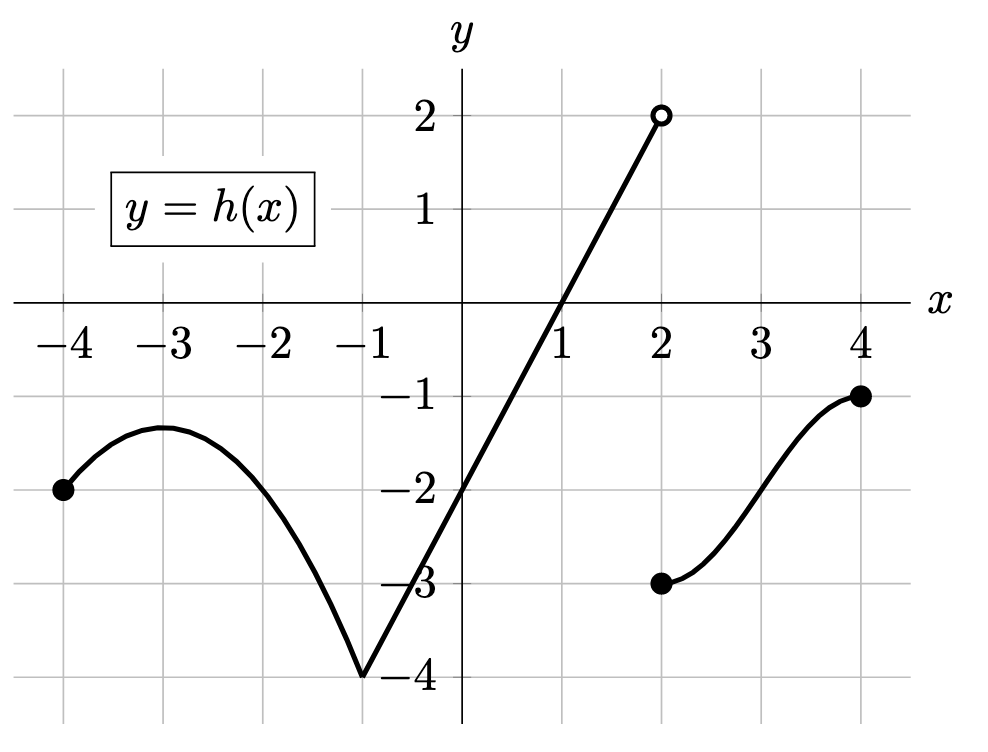
\includegraphics[scale=0.4]{Figures/graphh2}
        \end{center}
        Define the function \(k(x)\) such that \[
          k(x) =
          \begin{cases}
            h(x) & -4 \leq x < 1 \\
            A^2 \sin(Ax+B) & 1 \leq x \leq 4
          \end{cases}
        \]
        where \(A\) and \(B\) are constants. Find one pair of values for \(A\) and \(B\) that make \(k(x)\) differentiable
        at \(x = 1\). Show your work
        \begin{solution}
          See part (d) of \href{https://dhsp.math.lsa.umich.edu/exams/115exam2/f19/s7.pdf}{https://dhsp.math.lsa.umich.edu/exams/115exam2/f19/s7.pdf}
        \end{solution}
\question (Fall 2015 Exam 2) The graphs of two functions, \(h(p)\) and \(v(p)\), are shown below.
  \begin{center}
    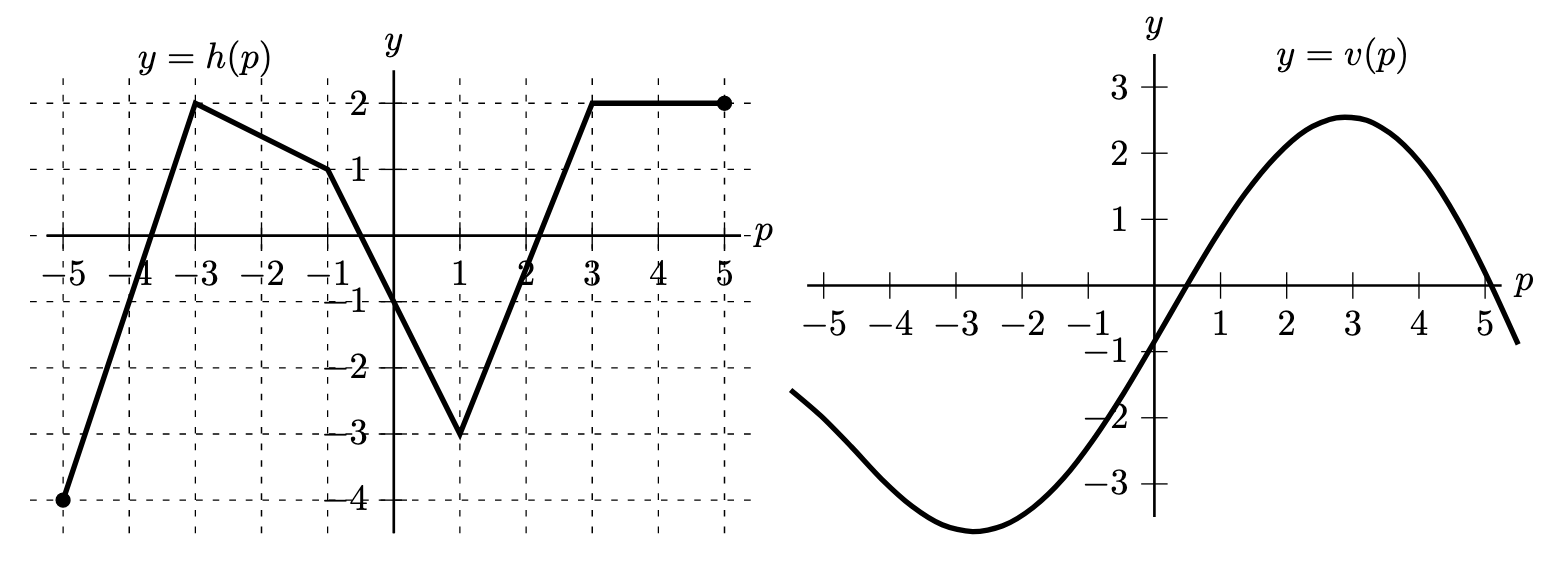
\includegraphics[scale=0.5]{Figures/Fall15Exam2p1}
  \end{center}
The following questions concern the functions \(B\), \(W\), and \(Q\) defined as
follows: \[
  B(p) = \frac{h(2p)}{h(4p)}, \qquad W(p) = h(h(p)), \qquad \text{and}\qquad Q(p) = e^{-v(p)}
\]
Assume that the first and second derivatives of \(v(p)\) are defined everywhere, i.e. that both \(v\)
and \(v'\) are differentiable on \((-\infty, \infty)\). Note that the graph of \(h(p)\) consists of line segments
whose endpoints have integer (whole number) coordinates. Find the exact value of each of
the quantities in (a) and (b). below. If the value does not exist, write does not exist.
Remember to show your work carefully.
\begin{parts}
\part \(B'(-1)\)
\part \(W'(2)\)
\part On the interval \(-2 < p < 2\), is \(Q(p)\) always increasing, always decreasing, or
neither? Show your work and explain your reasoning.
\end{parts}
\begin{solution}
  See \href{https://dhsp.math.lsa.umich.edu/exams/115exam2/f15/p1.pdf}{https://dhsp.math.lsa.umich.edu/exams/115exam2/f15/p1.pdf}
\end{solution}
\end{questions}
\end{document}
%%% Local Variables:
%%% mode: latex
%%% TeX-master: t
%%% End:
